\section{System overview}

We briefly introduce the considered supermarket setting and
detail our order picking pipeline and system components.

\subsection{Considered supermarket setting}

Modern supermarkets are characterized by a large range of
products, around 100,000 different products per store.
Operators usually have access to detailed information of all
those products, including mass, geometry, and shelf location
in the store. In our demonstration, we assume that the robot
can access this database to inform its decision. The large
variety of products usually requires specialized grasping
strategies per category, e.g., grasping tomatoes is
different from grasping a large soft\hyp{}drink bottle. We focus
on a subset of products that can be picked with the suction
gripper of our robot (see hardware design in
\cref{sec:hardware}), e.g., cans, milk boxes, bottles, or
bags of crisps (see \cref{fig:product_examples}). The masses
of products range from 100g (instant food mixes) to 1.5 kg
(soft\hyp{}drink bottle) and the size are between 10 cm (cans)
and 30 cm (soft\hyp{}drink bottle). We assume that products to
pick are visible, accessible from the shelf's front and in the robot's workspace.
\begin{figure}[t]
  \centering
  \begin{subfigure}[b]{0.24\linewidth}
    \centering
    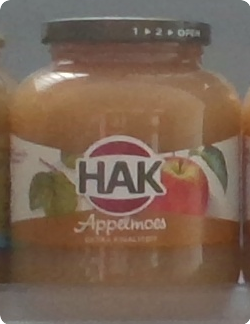
\includegraphics[height=1.2\textwidth]{appelmoes_rounded.png}
  \end{subfigure}%
  \begin{subfigure}[b]{0.24\linewidth}
    \centering
    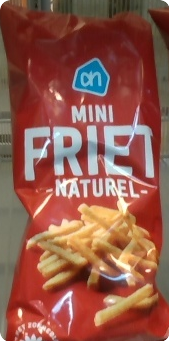
\includegraphics[height=1.2\textwidth]{fries_rounded.png}
  \end{subfigure}%
  \begin{subfigure}[b]{0.24\linewidth}
    \centering
    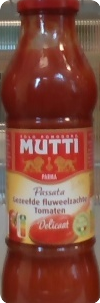
\includegraphics[height=1.2\textwidth]{mutti_rounded.png}
  \end{subfigure}%
  \begin{subfigure}[b]{0.24\linewidth}
    \centering
    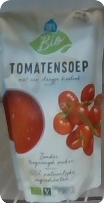
\includegraphics[height=1.2\textwidth]{soup_rounded.png}
  \end{subfigure}%
  \caption{Examples of different products considered in this
  work.}
  \label{fig:product_examples}
\end{figure}

%Moreover, in the interest of bridging the gap between robotics research and applications on the market, achieving high reliability for a part of all products is assumed to be favorable. Besides, 
For in\hyp{}store picking, we focus on picking products
during opening\hyp{}hours and favor reliability over execution speed. 
%, because warehouse automation is already being tackled by redesigning the interior making collaborative robots obsolete
%in such environments. Based on this focus, we generally favor reliability over execution speed. 

\subsection{Hardware}
\label{sec:hardware}

Our mobile manipulator platform is comprised of various hardware components. 

\paragraph{Robot}
The mobile manipulator is composed of two robots, see
\cref{fig:hardware}. The moving base is a Clearpath Boxer,
differential drive wheeled-robot that can achieve similar
speeds to humans while having a relatively small footprint.
The robotic arm is a
Franka Emika Panda, a serial manipulator with seven degrees
of freedom, equipped with torque sensors in every joint that
can achieve high accuarcy while being safe to work around,
see \cref{fig:layouts}. The attached gripper is a custom
3D-printed suction gripper with two suction cups powered by
a industrial vacuum pump.
\begin{figure}[t]
    \centering
    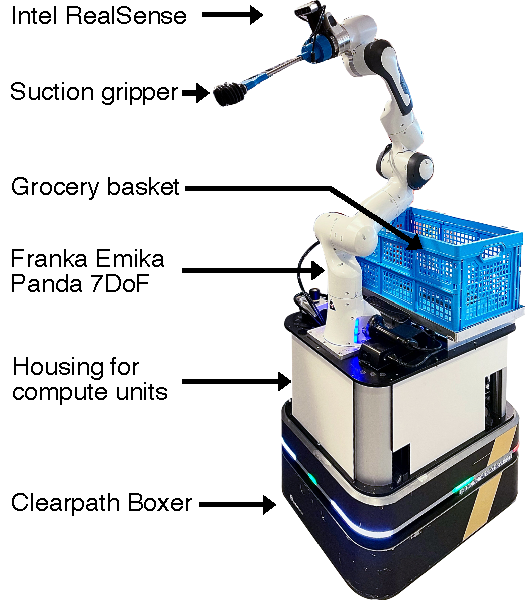
\includegraphics[width=0.65\linewidth]{AlbertHWIntro.pdf}
    \caption{Overview of our robot's hardware.}
    \label{fig:hardware}
\end{figure}


\paragraph{Perception}
The base uses a 270 degree Lidar sensor to localize itself
and detect dynamic obstacles and humans in the environment.
We mounted a Realsense D435 RGBD camera on the wrist link of
the arm and use it to detect products and perform visual
servoing during picking.

\paragraph{Compute Units}
We use a total of four compute units to distribute the computational load of individual software components. 
The first compute unit is the Franka Control Interface controlling the arm. 
The base's compute unit performs
self-localization and collision avoidance for the base.
The central compute
unit is an Intel NUC with an Intel i7 10th generation CPU, running all planning components and the user interface for placing orders. 
%Object detection and localization is
%running on an separate laptop mounted on the top of the robot, below the shopping
A Dell Alienware laptop mounted on the robot with an RTX 3070 TI GPU runs the perception components. %perform
%inference on the detector network and image processing.
Our two computers are running the Robot Operating System (ROS) and communicate via a network switch.


\subsection{Order\hyp{}picking overview}
\label{sec:order_system_overview}



\begin{figure*}[ht]
  \centering
  \begin{subfigure}[b]{0.18\linewidth}
    \centering
    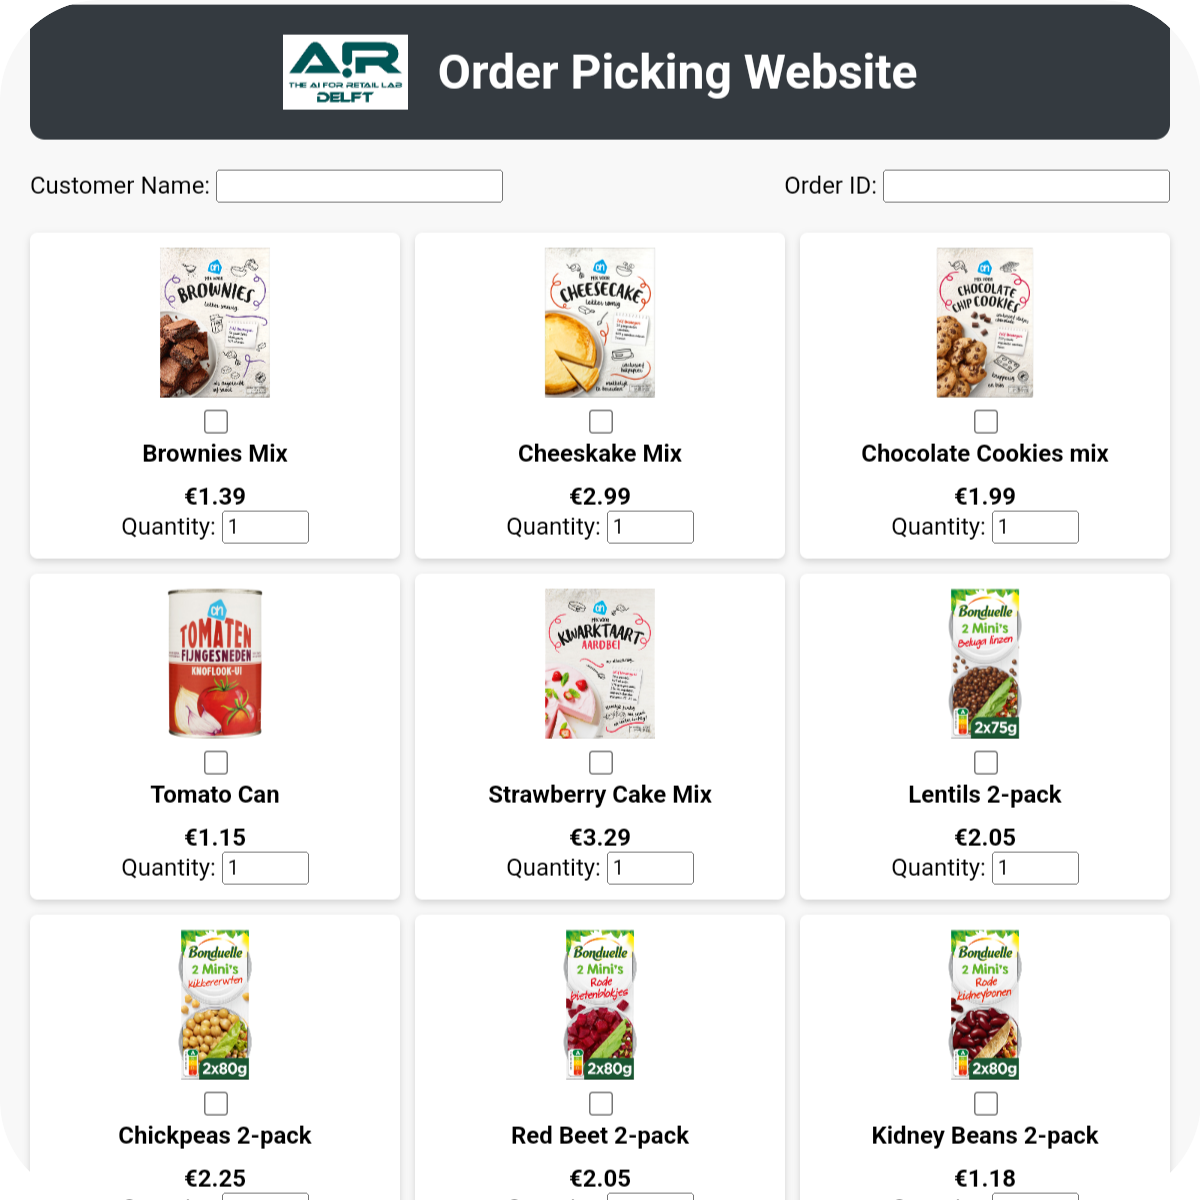
\includegraphics[width=1\textwidth]{order_interface.png}
    \caption{Customer order}
  \end{subfigure}%
  \begin{subfigure}[b]{0.18\linewidth}
    \centering
    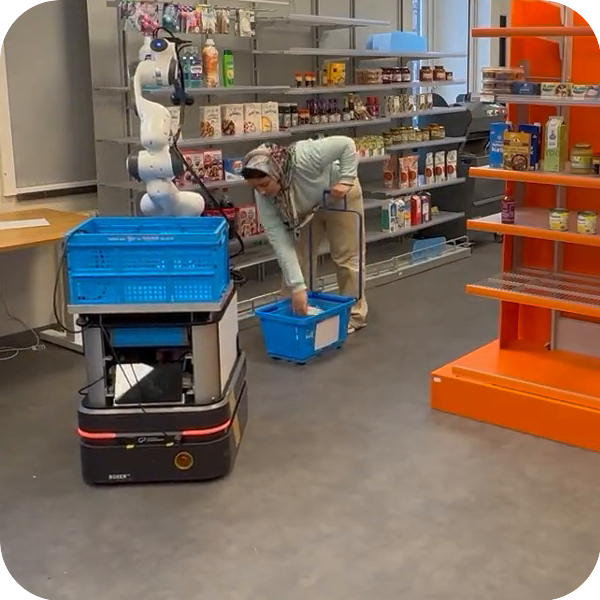
\includegraphics[width=1\textwidth]{navigation.png}
    \caption{Navigate to shelf}
  \end{subfigure}
  \begin{subfigure}[b]{0.18\linewidth}
    \centering
    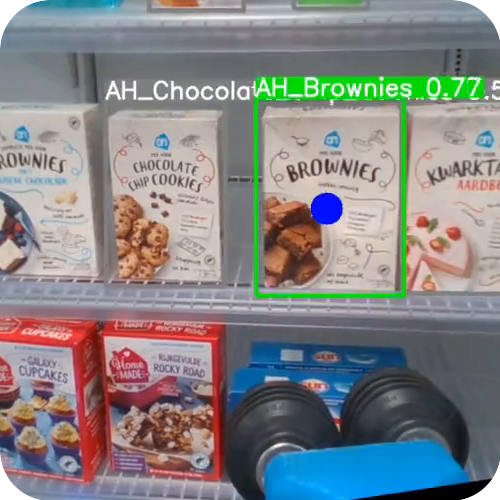
\includegraphics[width=1\textwidth]{locate_item.png}
    \caption{Locate item}
  \end{subfigure}
  \begin{subfigure}[b]{0.18\linewidth}
    \centering
    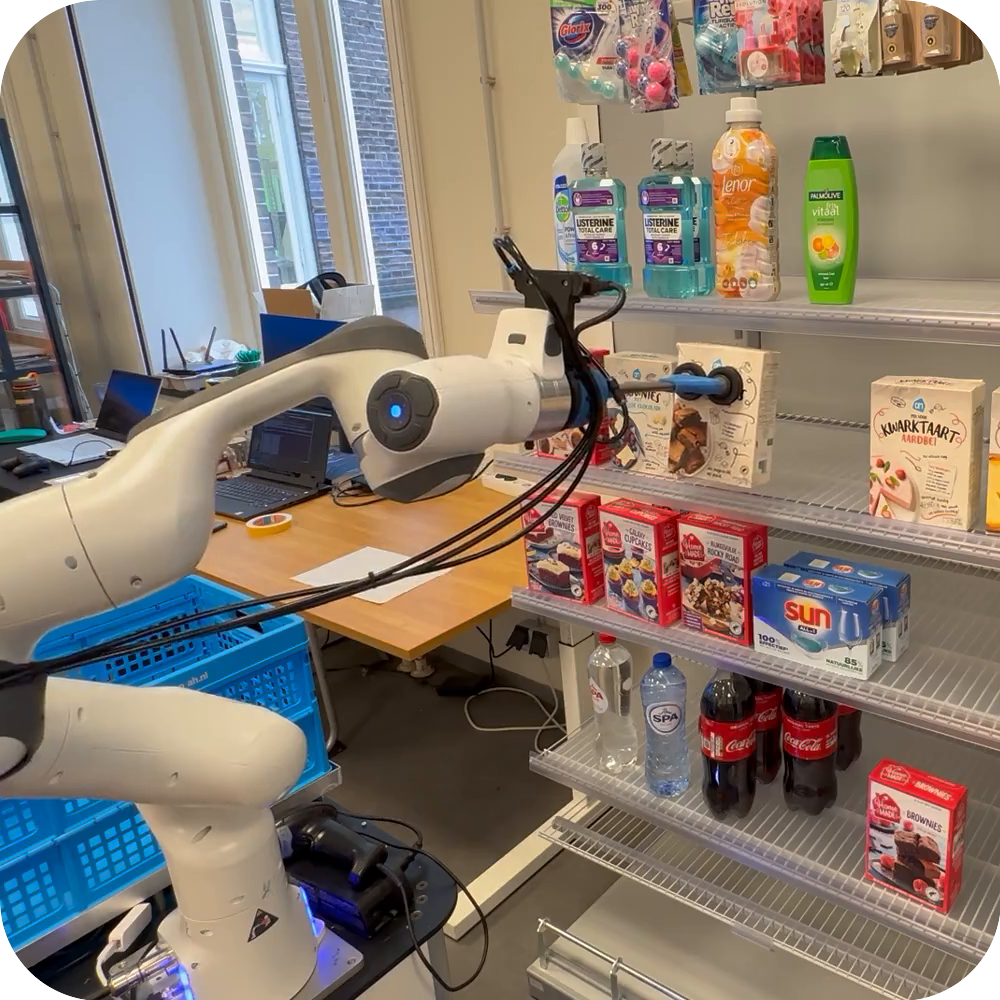
\includegraphics[width=1\textwidth]{picking.png}
    \caption{Pick item}
  \end{subfigure}
  \begin{subfigure}[b]{0.18\linewidth}
    \centering
    \includegraphics[width=1\textwidth]{placing.png}
    \caption{Place item}
  \end{subfigure}
  \caption{Overview of ideal flow of symbolic actions to complete an order.}
  \label{fig:flow}
\end{figure*}


%A static sequence of tasks for order-picking in supermarkets can roughly be described as follows.
%
The high\hyp{}level overview of our order\hyp{}picking system is
illustrated in \cref{fig:flow}.
Customers first place an order via the order placement website. 
The robot processes the order into a task assignment. 
For each item, it navigates to the item's shelf, locates it, picks and places it in the basket.
When the order is completed, the customer can pick up the order from the robot.





\subsection{System components}

We used the order\hyp{}picking sequence in \cref{sec:order_system_overview} to guide our system development, while focusing on adaptiveness to recover from failure and inaccuracies in perception. 
In the following, we outline the main
system components that are visualized in \cref{fig:software_overview} and can be grouped in: 
\begin{figure}[t]
  \begin{center}
    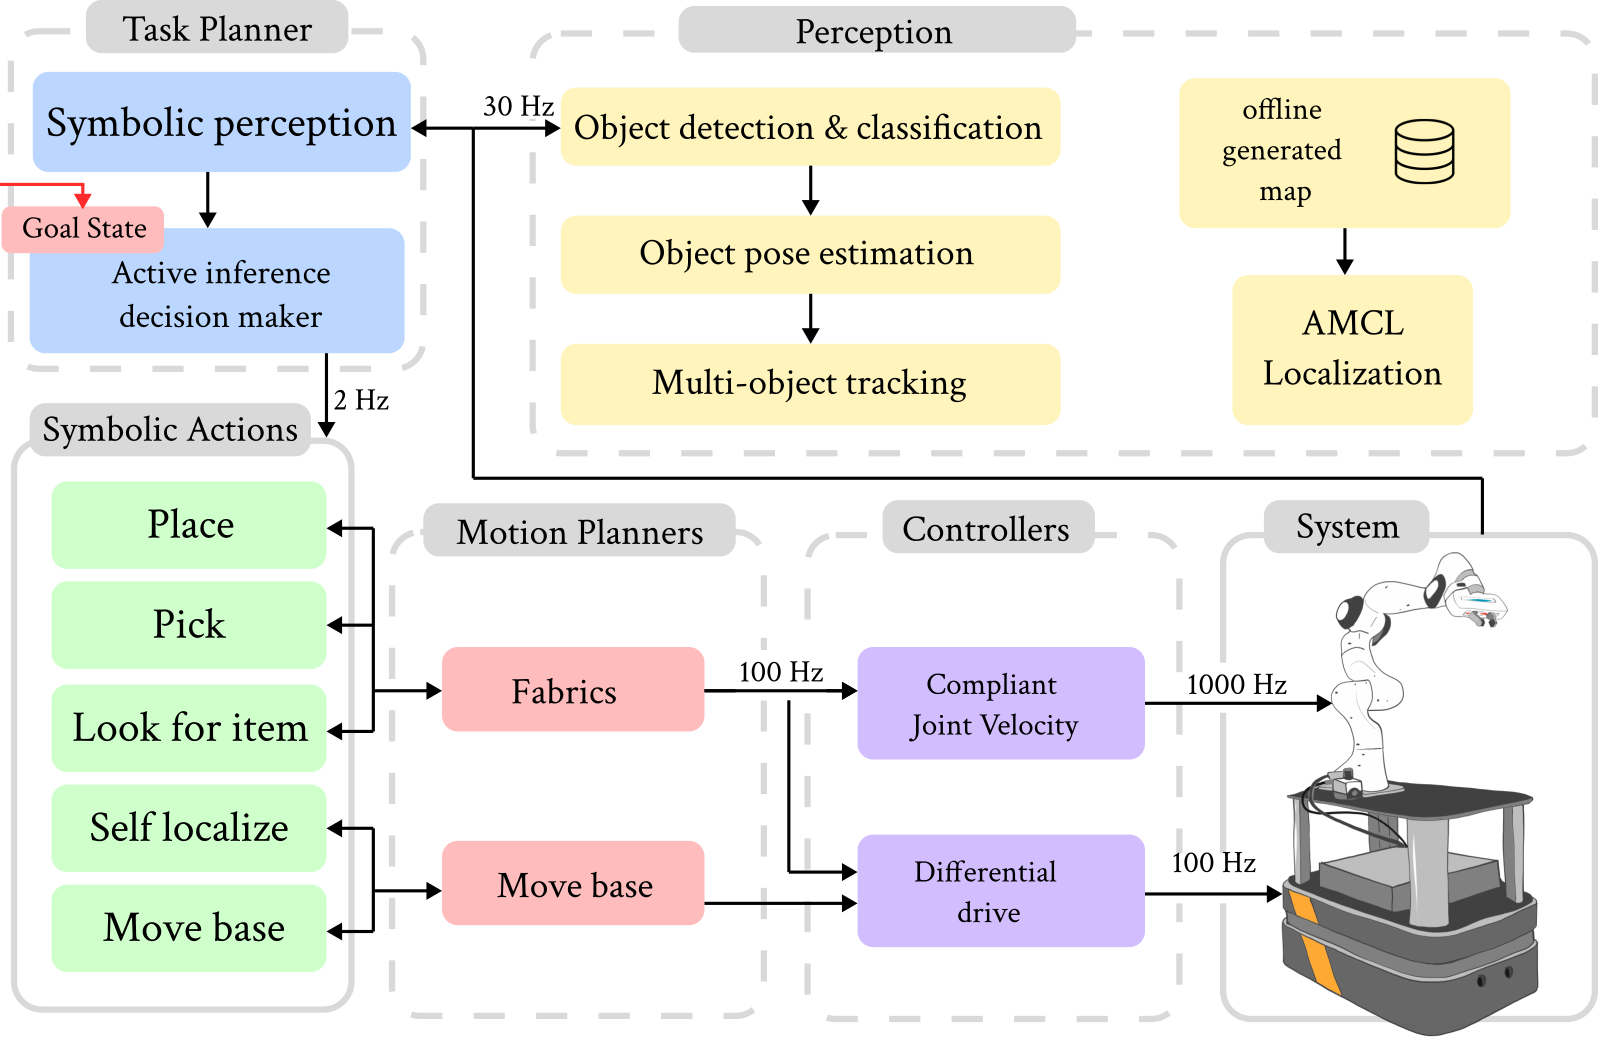
\includegraphics[width=1.00\linewidth]{overview_updated.png}
  \end{center}
  \caption{Overview of system components.}
  \label{fig:software_overview}
\end{figure}
%The overview of our system components is visualized in. 
(a) task planner, (b) motion planners, (c) low\hyp{}level controllers, and (d) perception.


After receiving the customer order, the task planner (see
\cref{sec:decision_making}) determines the order of picking
products by minimizing the robot's travelled distance. The
task planner uses a combination of a behavior tree and
symbolic state information, such as the robot is holding a
product or has arrived at the desired position,
with an adaptive inference method to determine the best next
symbolic action to execute.
We define a \textit{symbolic action} as an elementary robot
behavior. Symbolic actions can be as simple as greeting the
customer or as complex as picking an item.
We use a set of five robot
symbolic actions:
picking items, placing items, looking for items, localizing
the robot, and navigating the robot. Each symbolic action is realized
by the motion planning and control components (see
\cref{sec:trajectory_generation}). Motion planning is
decomposed into path planning and online trajectory
optimization for the base and reactive trajectory generation
for the arm, augmented with a pseudo\hyp{}prismatic joint on the
base, see \cref{sec:trajectory_generation}. Lastly, the
perception component (see \cref{sec:perception}) takes care
of item detection and classification and provides item poses
to the planning components.
